\chapter[The Effects of Increased NSB on the FD Trigger and Reconstruction]{\centering The Effects of \\ Increased Night Sky Background on \\ the Fluorescence Detector's Trigger and Reconstruction \\ }\label{Ch:SelectEff}


%Selection Efficiency of EAS under increased NSB
%\begin{itemize}
%\item Smearing real data with extra noise
%\item Simulating EAS with an increased NSB
%\item Talk about differences in smearing and simulating EAS (different triggering conditions)
%\item Energy and Xmas resolution and bias
%\item Rp bias
%\item differences in track length
%\end{itemize}

% Quantifying Effects of Increased Night Sky Background on Reconstruction and Detection of Extensive Air Showers

\section{Motivation}

The Pierre Auger Observatory has been operational since 2004 and the collaboration  is in the process of rolling out upgrades to improve operations. The upgrade has been name AugerPrime \textbf{(ref)} and is a large project to improve both the Surface Detectors (SD) and the Fluorescence Detectors (FD). The FD portion of AugerPrime involves extending the duty cycle to observe EAS events while the moon is above the horizon. The main purpose of this is for the collaboration to be able to collect more EAS events in the highest energy bin ($>$ 10$^{19.5}$ eV). 

In this chapter I used real data and simulations to explore the effects of increasing the Night Sky Background on the collaboration's reconstruction method and trigger efficiency .A real data set was used to evaluate the efficiency of the reconstruction method under different NSB levels by artificially adding extra noise to signal traces. This was a repetition of a study done by M. Unger \textbf{Find ref.} which was used as a starting point and then was expanded on. The expanded work lead to using simulations to evaluate the full trigger and reconstruction efficiency. The Efficiency was calculated with he equation used is:
\begin{equation}
\mathrm{Efficiency} = \mathrm{N}^{'}_{\mathrm{Select}} \ / \ \mathrm{N}^0_{\mathrm{Select}}
\end{equation}
where $\mathrm{N}^{0}_{\mathrm{Select}}$ is the number of selected events at the standard NSB level and $\mathrm{N}^{'}_{\mathrm{Select}}$ is the number of selected events at the increased NSB
level. 

After the Efficiency was calculated the bias and resolution for Xmax and energy was determined. For real data, the bias is the relative change in the mean of the distributions at increased NSB to the mean of the distributions at standard NSB, both after reconstruction and selection cuts. The bias calculations for real data become:
\begin{eqnarray}
\Delta \mathrm{E}_{\mathrm{Data}} &=& \frac{\mathrm{E}_{\mathrm{IncreasedNSB}} - \mathrm{E}_{\mathrm{StandardNSB}}}{\mathrm{E}_{\mathrm{StandardNSB}}} \label{eq:energybias_data} \\
\Delta \mathrm{Xmax}_{\mathrm{Data}} &=& \mathrm{Xmax}_{\mathrm{IncreasedNSB}} - \mathrm{Xmax}_{\mathrm{StandardNSB}}\label{eq:xmaxbias_data}
\end{eqnarray} 
For simulated data the bias is the relative change in the mean of the distributions after the full simulation by EAS events going through an atmosphere with a specified NSB photon field, the FD telescopes optics, trigger, reconstruction and selection cuts compared with Monte-Carlo truth.
\begin{eqnarray}
\Delta \mathrm{E}_{\mathrm{Sim}} &=& \frac{\mathrm{E}_{\mathrm{recon}} - \mathrm{E}_{\mathrm{true}}}{\mathrm{E}_{\mathrm{true}}}  \label{eq:energybias_sim} \\
\Delta \mathrm{Xmax}_{\mathrm{Sim}} &=& \mathrm{Xmax}_{\mathrm{recon}} - \mathrm{Xmax}_{\mathrm{true}} \label{eq:xmaxbias_sim}
\end{eqnarray}
 
 
The energy and Xmax resolution is calculated via:
\begin{eqnarray}
\sigma_{\mathrm{res}} &=& \left( \frac{1}{\mathrm{N}} \sum \frac{1}{\sigma^2_i} \right)^{1/2}
\end{eqnarray}





Currently the Fluorescence Detectors (FDs) are operated under these guidelines: an observation run is organised for nights when the illuminated fraction of the moon less then 70\% and can have a minimum of 3 hours of operation with the moon below the horizon. The FD telescope shutters are then opened when the sun is below -18\textdegree \ of the horizon (beginning of astronomical twilight). The FD shutters remain open while the average variance across the FD camera is less then 100 ADC$^2$/100 ns and the variance of individual PMTs is less then 2000 ADC$^2$/100 ns. The FD shutters at each site will also close if the individual rain sensors are trigger or the measured wind speed is above 50 km/h.  From these guidelines the FD time of operation can be calculated. A calculation performed by the collaboration to estimate the theoretical up time of the FD's was done before 2012 \textbf{(find ref.)} in Table \ref{tab:CFD_Q_F}.
\begin{table}[h]
\centering
\begin{tabular}{c c}
\hline\hline
Theoretical up time & 22\% \\
Loss due to short nights ($<$ 3 hrs) & -2\% \\
Loss due to bad weather or failures & -5\% \\ \hline \hline
Total measurement time & 15\% \\
\hline\hline
\end{tabular}
\caption{Calculation of the FD up-time done by the Colabration. Bad weather is the inclusion of rain, high wind speeds and lightning strikes in the FDs field of view. Explain Failure - equipment not working.} \label{tab:FD_uptime}
\end{table}
For context, the ADC$^2$/100 ns measured by the FD PMTs at standard operation typically observe Night Sky Background (NSB) with no moon, quarter moon and full moon/twilight are shown in Table \ref{tab:MoonLightADC}. Bad weather is the inclusion of rain, high wind speeds and lightning strikes in the FDs field of view.
\begin{table}[h]
\centering
\begin{tabular}{c c c}
\hline\hline
Condition & $\sigma^2$ [ADC$^2$/100 ns] & I$_{\mathrm{a}}$ [$\mu$A] \\ \hline\hline
no moon & 25 & 0.5 \\
quarter moon & 250 & 5 \\
full moon/twilight & 2500 & 50 \\ 
\hline\hline
\end{tabular}
\caption{Expected average observed variance in ADC$^2$ and anode current in $\mu$A by the PMTs in the FD telescopes under different NSB conditions. No Moon is the typical conditions that the FD shift is run under.  } \label{tab:MoonLightADC}
\end{table}

The PMTs used as camera pixels are XP3062 and are operated at a gain of $\sim$ 5 $\times$ 10$^4$ electrons/photo-electron which give the above values in the table. The datasheet \textbf{(find ref.)} for the XP3062 recommend that for good stability anode currents less than 10 $\mu$A be measured. 
  


Later within this thesis I will investigate the effects of lower the gain on the PMTs to reduce the measured anode current. A lower anode current when observing under moonlight would help make sure that the PMT lifespans are not changed by the increased in NSB. A PMT lifetime is measured in the amount of anode current removed in operation. A reduced gain by a factor of ten would theoretical allow the operation of the PMTs while a quarter moon is above the horizon in the same way as the current PMT operation.  

The signal that the FD's observe is AC coupled, which means the mean signal of the NSB is zero. Instead the variance around zero is calculated and is directly proportional to the fluctuations in the NSB. The average value of the NSB measured by Auger at Malargue is:
\begin{equation}
\sigma^2 \sim 25 \ \mathrm{ADC}^2 \ / \ 100 \mathrm{ns}
\end{equation}
The variance in ADC$^2$ can be converted into photons seen at the aperture by using:
\begin{eqnarray}
\sigma^2_{pe} &=& [\sigma^2_{\mathrm{ADC}}]^{\mathrm{sky}} \ / \ \mathrm{A}^2_{\mathrm{G}} \label{eq:simgaPE} \\
\mathrm{n}_{\mathrm{ph}} &=& \frac{\sigma^2_{pe}}{(1 + \mathrm{V}_{\mathrm{G}})} \label{eq:numPhoton}
\end{eqnarray}
where $\sigma_{pe}$ is the standard deviation of the photo-electron count, n$_{\mathrm{ph}}$ is the photon count and A$_{\mathrm{G}}$ is equal to:
\begin{equation}\label{eq:abs_gain}
\mathrm{A}_{\mathrm{G}} = \frac{1}{\mathrm{C}_{\mathrm{FD}}.\mathrm{f}.\mathrm{Q}}
\end{equation}
where
\begin{itemize}
\item[] A$_{\mathrm{G}}$ is the absolute gain (ADC/photo-electron)
\item[] $\mathrm{C}_{\mathrm{FD}}$ is the FD pixel calibration constant.
\item[] Q is the Quantum efficiency of the PMT turning photons into photo-electrons.
\item[] f is the photon collection efficiency of the telescope optics.
\end{itemize}

/*------ \textbf{Find reference to number below} ------*/

Typical measured values for C$_{\mathrm{FD}}$, Q and f shown in Table \ref{tab:CFD_Q_F}.
\vspace{3mm}
\begin{table}[h]
\begin{center}
\begin{tabular}{|c|c|}
\hline 
C$_{\mathrm{FD}}$ & 4.5 photons/ADC \\
\hline
Q & 0.29 \\
\hline
f & 0.465 \\
\hline
\end{tabular} 
\end{center}
\caption{Typical values for the constants use to calculate A$_{\mathrm{G}}$ which is the absolute gain (ADC/photo-electron). $\mathrm{C}_{\mathrm{FD}}$ is the FD pixel calibration constant, Q is the Quantum efficiency of the PMT turning photons into photo-electrons and f is the photon collection efficiency of the telescope optics.} \label{tab:CFD_Q_F}
\end{table} 

Therefore A$_{\mathrm{G}}$ can be calculated from Eq. \ref{eq:abs_gain} and using the values from Table \ref{tab:CFD_Q_F}. If $\sigma^2_{\mathrm{ADC}}$ = 25 ADC$^2$ / 100 ns, through the calculations n$_{\mathrm{ph}}$ = 23 photons / 100 ns. The calculations to work out the RMS$_{\mathrm{ph}}$ from the measured variance in ADC$^2$ is as follows:
\begin{equation}
\mathrm{RMS}_{\mathrm{ph}} = \mathrm{C}_{\mathrm{FD}} \times \sqrt{\mathrm{ADC}^2}
\end{equation}
From all of the equations stated above I have outlined a table showing the expected photon count at the aperture per 100 ns from the measured variance (ADC$^2$ / 100 ns).
\begin{center}
\begin{tabular}{| c | c | c | c |}
\hline \hline
\textbf{Variance} & \multirow{2}{*}{\textbf{log$_{10}$(V/ADC$^2$)}} & \multirow{2}{*}{\textbf{Photons/100 ns}} & \textbf{RMS} \\
\textbf{(ADC$^2$ / 100 ns)} & & & \textbf{(Photons/100 ns)} \\
\hline \hline
25 & 1.40 & 22.7 & 22.5 \\
\hline
178 & 2.25 & 161.4 & 60 \\
\hline
259 & 2.40 & 226.7 & 71.2 \\
\hline
1000 & 3.00 & 907.0 & 142.3 \\
\hline
\end{tabular}
\end{center}


- Need graph of expected variance in ADC$^2$ / 100 ns for the moon above the horizon for different phases.

- Want to increase the duty cycle of FD by measuring EAS under moonlight. Most likely observe under quarter to half moon. This will increased the NSB up to a factor of 10.

- The aim of increasing the duty cycle of FD is too measure more EAS at the highest energy band ($> 10^{19.5}$ eV).

- Need more statistics at highest energy band to complement SD measurements.


\section{Selection Efficiency}

I investigated evaluating increasing the NSB by different factors on event reconstruction seen the FD's through a couple of different methods. The main increase of NSB will from observing while the moon is above the horizon. The two methods involved simulating increased NSB on measured data and with simulating. The measured data had increased noise introduced across the entire signal trace and I have labelled as the smearing method.

Selection Efficiency for the two methods are calculated via:
\begin{equation}
\mathrm{Efficiency} = \mathrm{N}_{\mathrm{Selected}} / \mathrm{N}_{\mathrm{total}}
\end{equation}
where for the Smearing method N$_{\mathrm{total}}$ is the total number of measured EAS events at standard NSB levels and N$_{\mathrm{Selected}}$ is the number of events after being reconstructed and passing the quality cuts with the increased NSB. For the simulations, N$_{\mathrm{total}}$ is the total number of simulated events before \textbf{need to check whether its the number of simulations before triggering or number of triggered events at standard NSB. Pretty sure the comparison is done with no. of simulated event at standard NSB}.

Smearing method involves taking the raw fluorescence telescope EAS shower events that would passed reconstruction and quality cuts and adding addition variance in ADC$^2$ equivalent to an increased NSB from moonlight to the FD pixel signal traces. The shower events are then reconstructed and passed through the same quality cuts. This a repartition of a similar method that M. Unger had preformed in \textbf{2012}. \textbf{Also need to refer to the study done by Brue and Andrew Smith around 1999}. This was done so a deeper analysis could be preformed to understand the underlying mechanics. 

The simulations were done using the simulation modules for the FD's within the $\overline{\mathrm{Off}}$\underline{Line} analysis programs. The EAS profiles were generated within CONEX and the original showers were generated through CORSIKA. The NSB was added to the EAS profiles before the FD are triggered. A hybrid trigger is used to involve the SD but the SD is simulated in a simple way just to get a simulated core position.

The smearing method was originally used as a proof of concept to show that EAS showers could still be reconstructed with the increased NSB. The limitation was that EAS were used that already triggered the FD's normally. The full simulation using CONEX showers was used to full test trigger conditions through to reconstruction. The simulations are not an 100\% accurate representation of the POA array so that will introduce some differences too.


\begin{figure}[!hp]
\centering
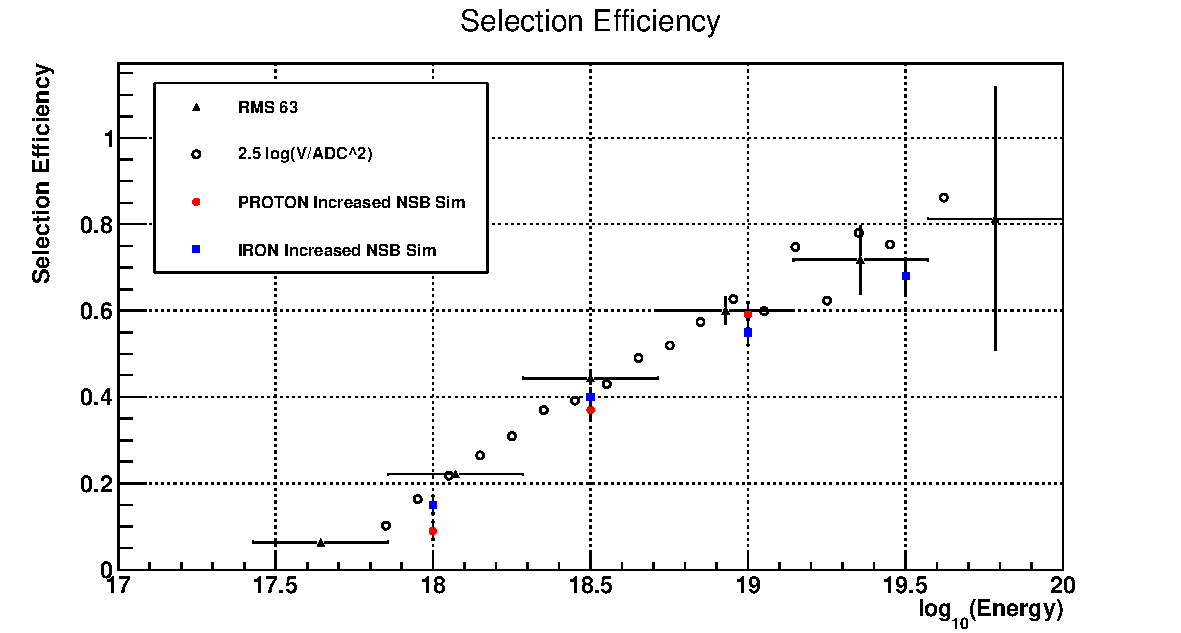
\includegraphics[width=\textwidth]{chapters/graphs/SelectionEff/SelectionEff_errorbars_10timesNSB.pdf}
\caption{Selection Efficiency plot containing data from both the Smearing method and simulated showers. These results are compared to the work done by M. Unger.}
\end{figure}

\section{Resolution and Bias}

To further evaluate the effects of increasing the NSB on the quality of the reconstructed EAS data, I look at the resolution and bias of both the reconstructed energy and reconstructed Xmax. A quick reminder that Xmax is the measurement of the brightest part of the shower relating to the maximum number of particles produced. For the smearing method the energy and Xmax bias is comparing to the measured data taken at standard NSB levels to the reconstructed with the increased NSB levels. For the simulations the energy and Xmax bias can be calculated using the true energy and Xmax values used to generate each EAS profile.

The trend of the energy resolution for both methods is that as the energy of the EAS event increases the bias decreases. This was expected as the energy of the shower increases the brighter and longer the track that is observed. A brighter and longer track allows for a better reconstruction.

- Need to find out what's a good bias value for energy and Xmax.

the energy and Xamx bias is calcualted via:
\begin{eqnarray}
\Delta \mathrm{E} &=& \frac{\mathrm{E}_{\mathrm{recon}} - \mathrm{E}_{\mathrm{true}}}{\mathrm{E}_{\mathrm{true}}}  \label{eq:energybias_sim} \\
\Delta \mathrm{E} &=& \frac{\mathrm{E}_{\mathrm{IncreasedNSB}} - \mathrm{E}_{\mathrm{StandardNSB}}}{\mathrm{E}_{\mathrm{StandardNSB}}} \label{eq:energybias_data} \\
\Delta \mathrm{Xmax} &=& \mathrm{Xmax}_{\mathrm{recon}} - \mathrm{Xmax}_{\mathrm{true}} \label{eq:xmaxbias_sim} \\
\Delta \mathrm{Xmax} &=& \mathrm{Xmax}_{\mathrm{IncreasedNSB}} - \mathrm{Xmax}_{\mathrm{StandardNSB}}\label{eq:xmaxbias_data}
\end{eqnarray}
Eq. \ref{eq:energybias_sim} and Eq. \ref{eq:xmaxbias_sim} are used on the simulated data sets while Eq. \ref{eq:energybias_data} and Eq. \ref{eq:xmaxbias_data} is used on the smeared data set.

The energy and Xmax resolution is calculated via:
\begin{eqnarray}
\sigma_{\mathrm{res}} &=& \left( \frac{1}{\mathrm{N}} \sum \frac{1}{\sigma^2_i} \right)^{1/2}
\end{eqnarray}


\begin{figure}
\centering
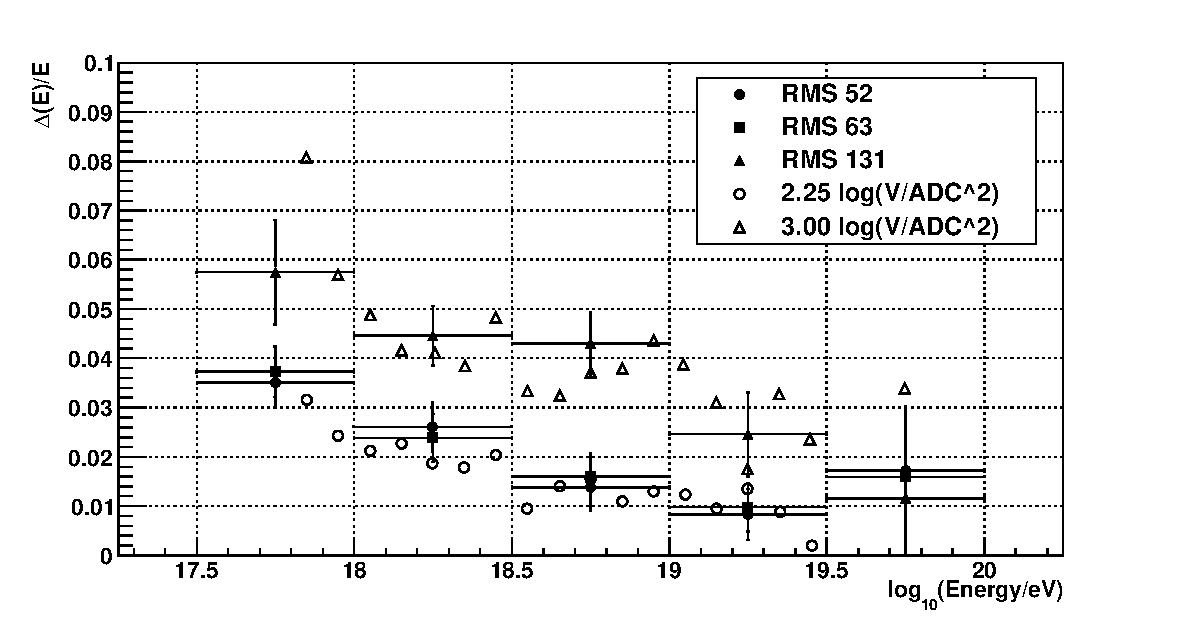
\includegraphics[width=\textwidth]{chapters/graphs/SelectionEff/Smearing_RealData_EnergyBias.pdf}
\caption{Energy Bias using Smearing Method.}
\vspace{3mm}
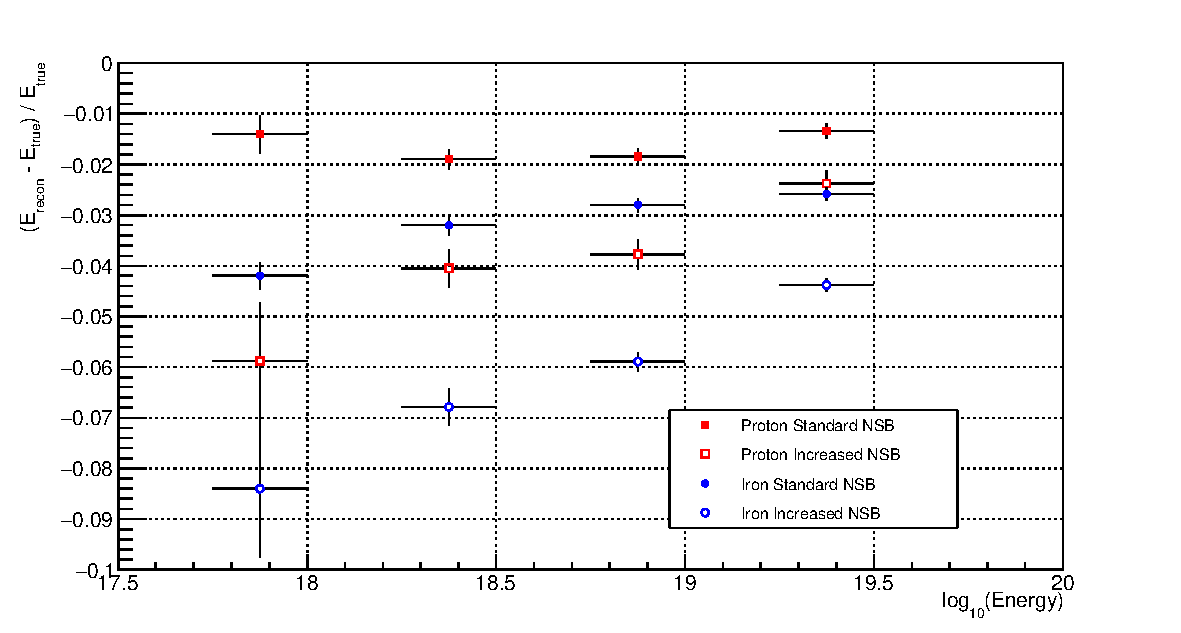
\includegraphics[width=\textwidth]{chapters/graphs/SelectionEff/Simulation_ProtonIron_EnergyBias.pdf}
\caption{Energy Bias using simulated data.}
\end{figure}

\begin{figure}
\centering
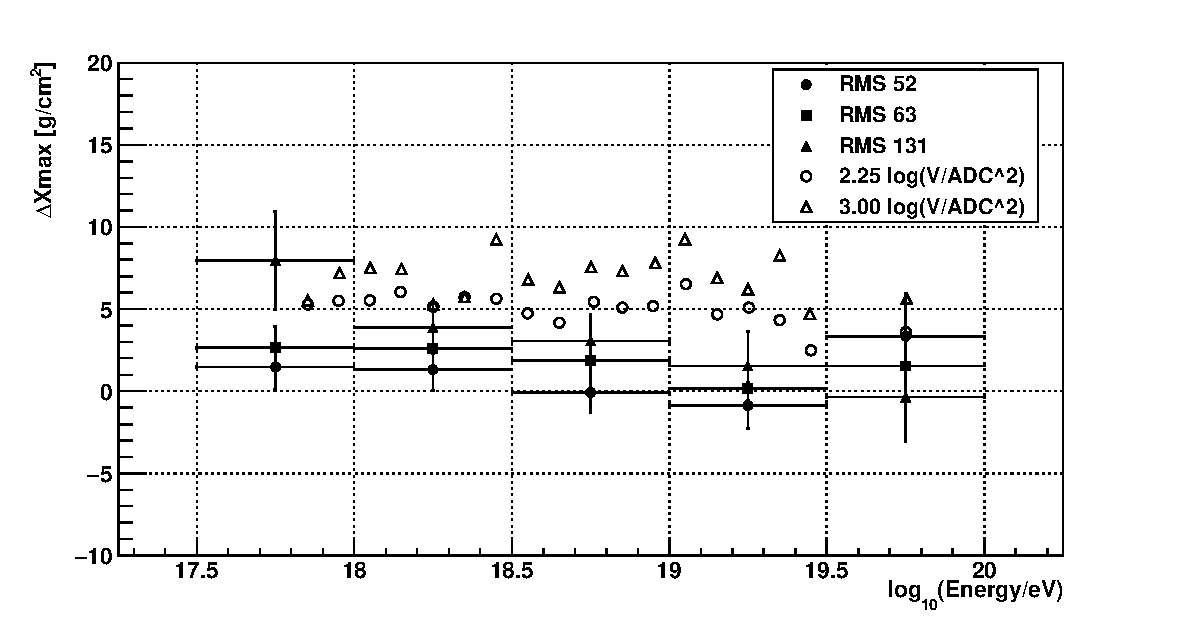
\includegraphics[width=\textwidth]{chapters/graphs/SelectionEff/Smearing_RealData_XmaxBias.pdf}
\caption{Xmax Bias using Smearing Method.}
\vspace{3mm}
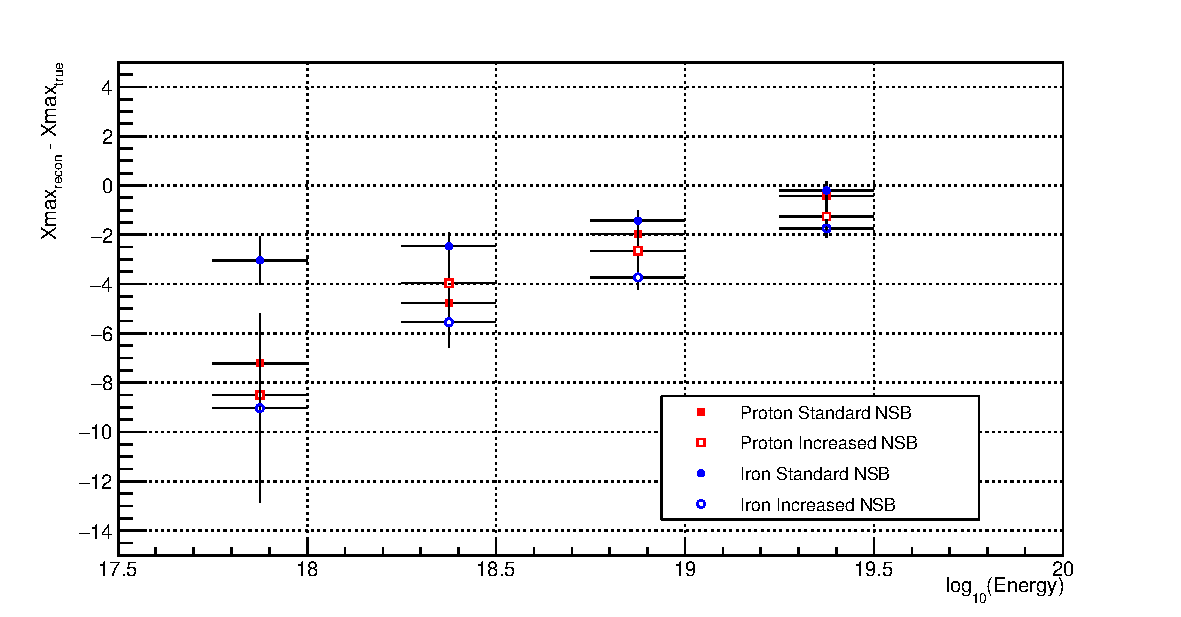
\includegraphics[width=\textwidth]{chapters/graphs/SelectionEff/Simulation_ProtonIron_XmaxBias.pdf}
\caption{Xmax Bias using simulated data.}
\end{figure}

\begin{figure}
\centering
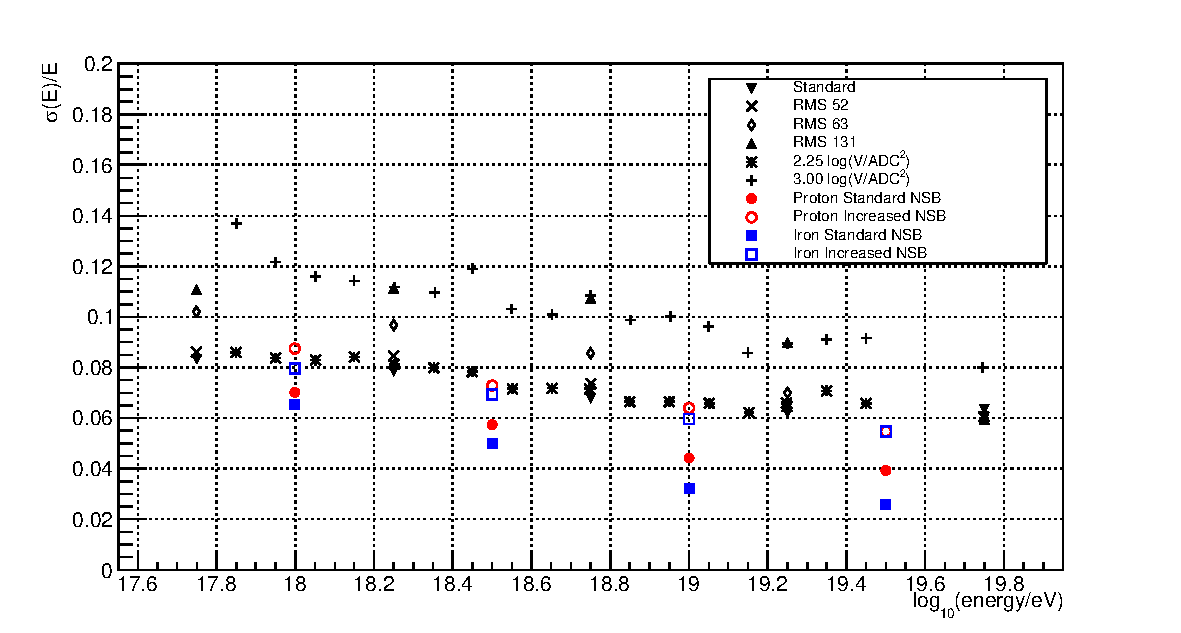
\includegraphics[width=\textwidth]{chapters/graphs/SelectionEff/Combined_EnergyRes_All.pdf}
\caption{Energy Resolution using both Smearing Method data and simulated showers.}
\vspace{3mm}
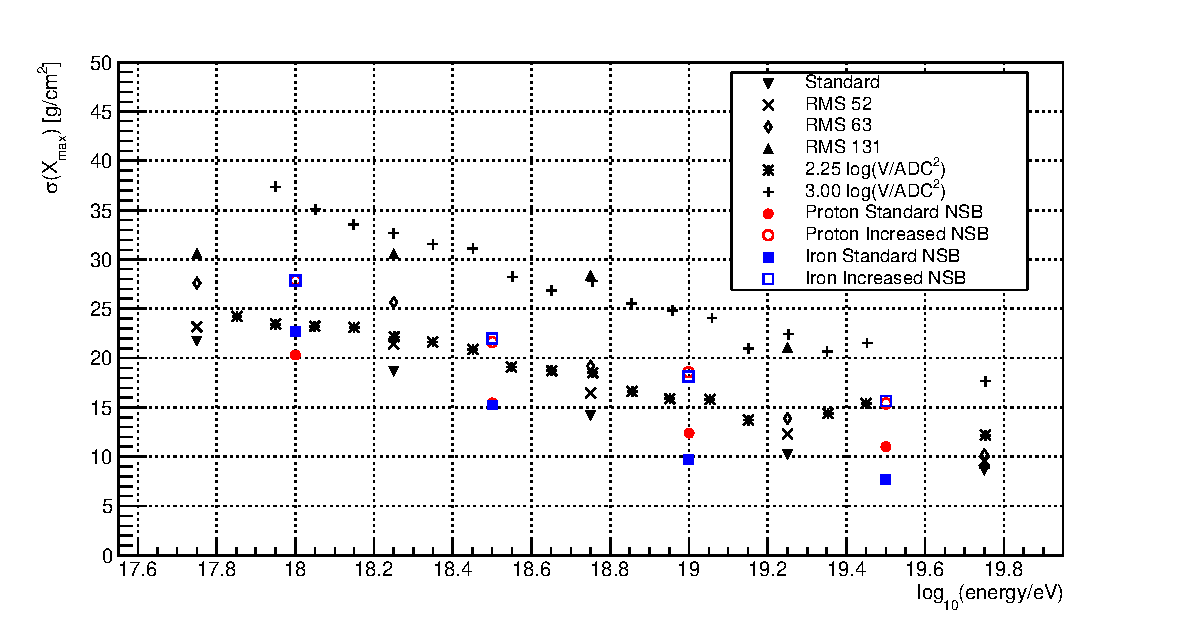
\includegraphics[width=\textwidth]{chapters/graphs/SelectionEff/Combined_XmaxRes_All.pdf}
\caption{Xmax Resolution using both Smearing Method data and simulated showers.}
\end{figure}

\subsection{Comparing Simulated Data to Real Data}

\textbf{Think about where to locate this section.}

Comparing the simulated data with real data. Checking to make sure that the simulation data is a good representation of reality. Looking at the Xmax distribution there is no need for a direction comparison as I only simulated proton and iron primaries and was not concern with have a particular mixtures. The other parameter I checked was the zenith angle distribution, distance to Xmax and distance to the shower axis (R$_{\mathrm{P}}$). The simulated profiles have similar shapes when both histograms are normalised to area of 1. For zenith angle distribution I simulated the EAS events upto a zenith angle of 60\textdegree so that the reason for the cut-off in the simulated data.

\begin{figure}
\centering
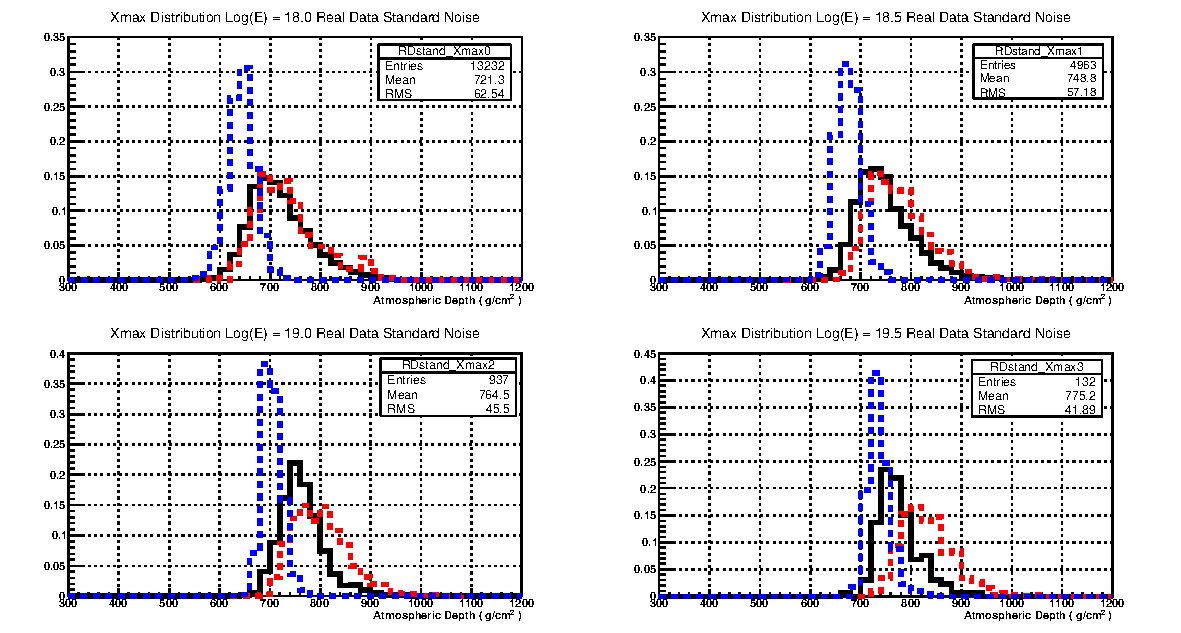
\includegraphics[width=\textwidth]{chapters/graphs/SelectionEff/RealDataAndSim_XmaxDistComp.pdf}
\caption{Distribution of Xmax with Real Data and simulation of proton and iron showers.}
\vspace{3mm}
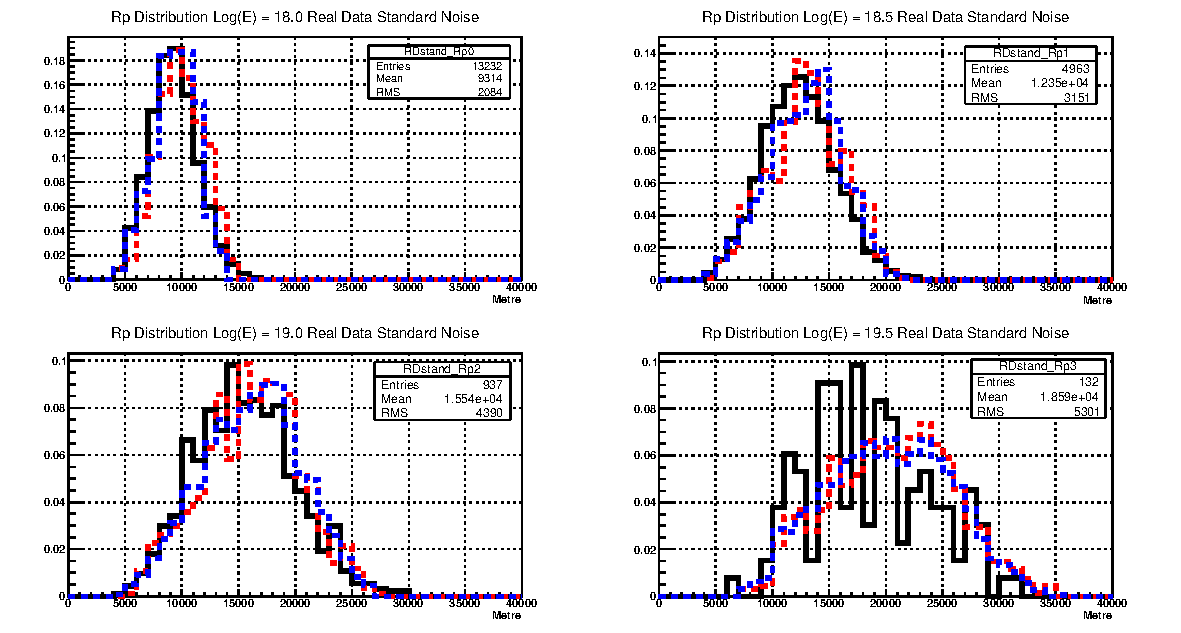
\includegraphics[width=\textwidth]{chapters/graphs/SelectionEff/RealDataAndSim_RpDistComp.pdf}
\caption{Distribution of Rp with Real Data and simulation of proton and iron showers.}
\end{figure}

\begin{figure}
\centering
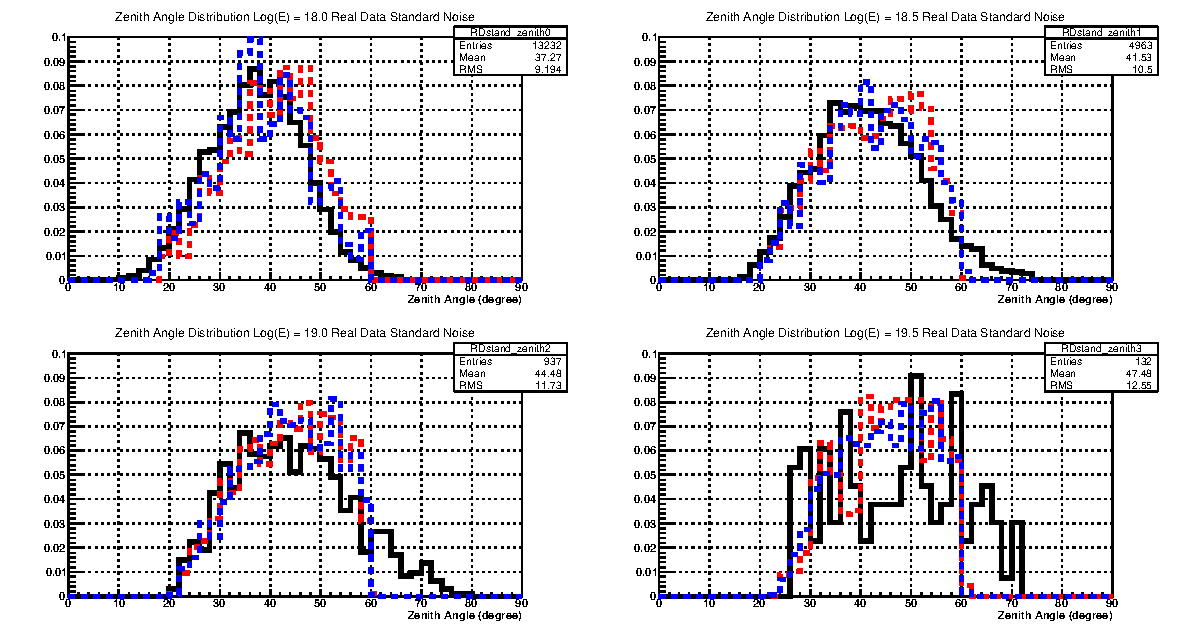
\includegraphics[width=\textwidth]{chapters/graphs/SelectionEff/RealDataAndSim_ZenithDistComp.pdf}
\caption{Distribution of Zenith angle with Real Data and simulation of proton and iron showers.}
\vspace{3mm}
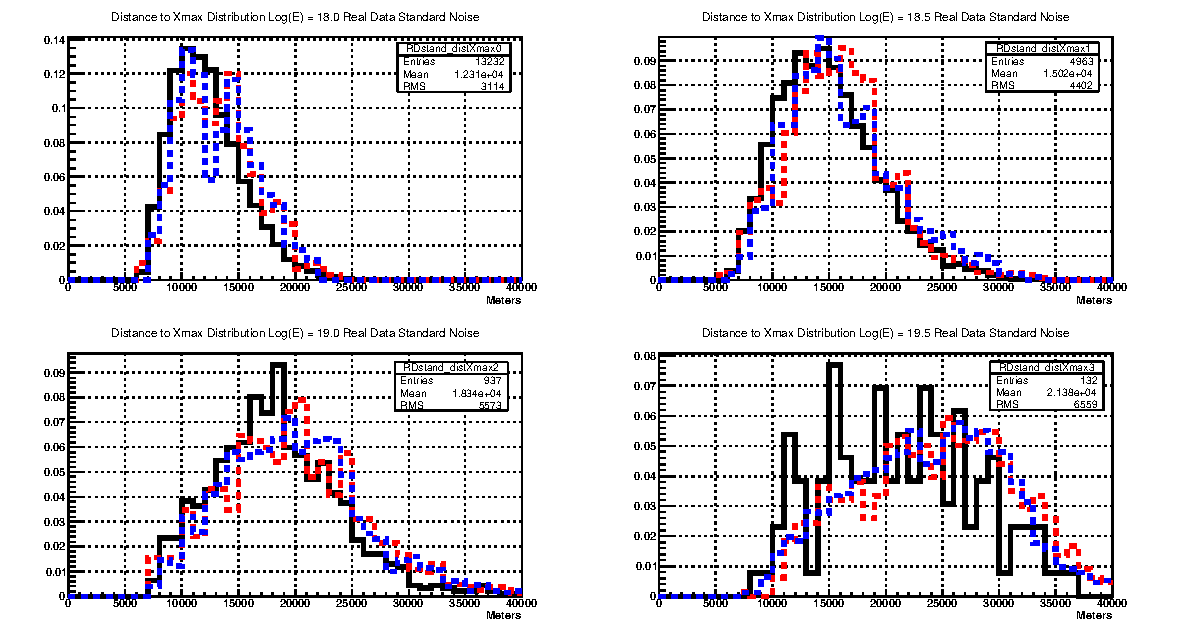
\includegraphics[width=\textwidth]{chapters/graphs/SelectionEff/RealDataAndSim_DistToXmaxDistComp.pdf}
\caption{Distribution of Distance to Xmax with Real Data and simulation of proton and iron showers.}
\end{figure}

\section{EAS Track Length in the FD's}

One other parameter that was investigate was the shower track length observed by the FD's. It was expected that as the NSB increased the average observed shower track length would decrease. For both the smearing and simulation this trend was observed by not in a significant way. This is shown in Fig. \ref{fig:TrackLength_Smearing} and Fig. \ref{fig:TrackLength_Sim}.  There was a thought about trying to extended track length into the noisy pixels as it would be known that would be photons observed at the start and end of the track. The measured data shows that this is not needed as not much of the track is lost with increased NSB. Especially at the highest energy bins where the most interest lays. 

\begin{figure}
\centering
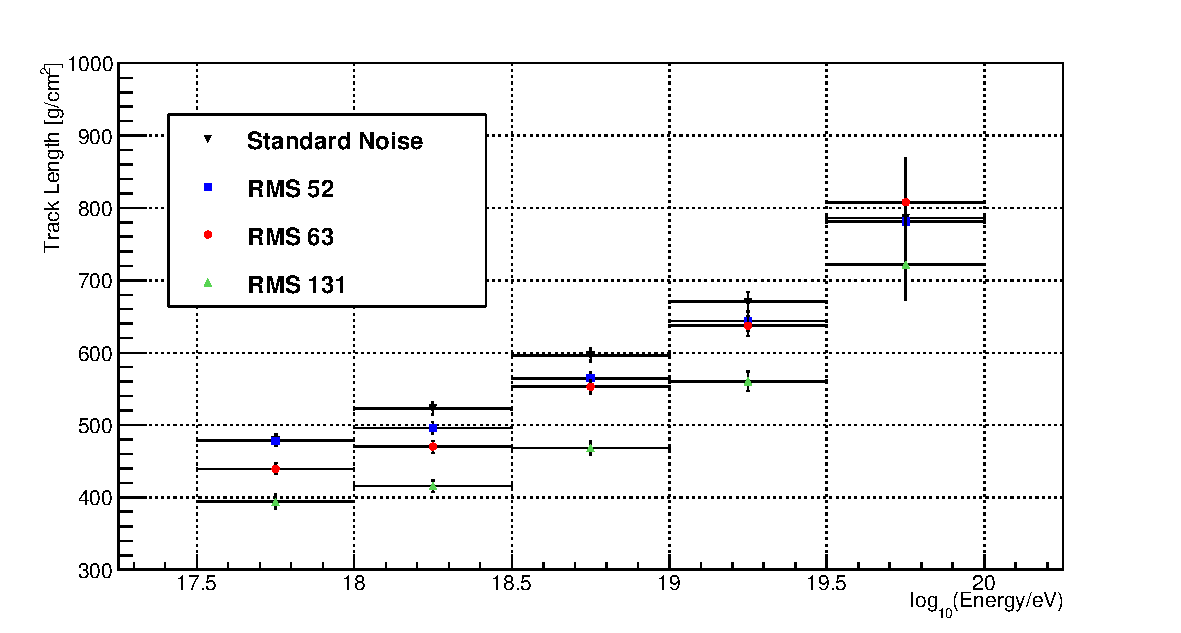
\includegraphics[width=\textwidth]{chapters/graphs/SelectionEff/Smearing_TrackLength_DiffNSBlevels.pdf}
\caption{Track length using Smearing method.} \label{fig:TrackLength_Smearing}
\vspace{3mm}
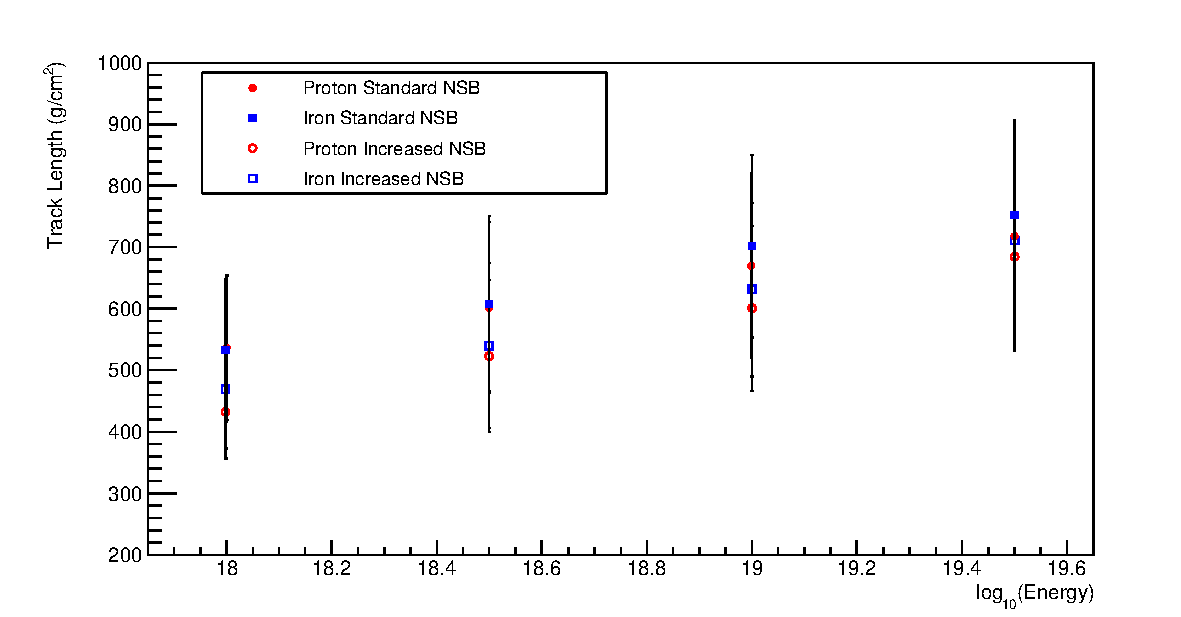
\includegraphics[width=\textwidth]{chapters/graphs/SelectionEff/Simulation_TrackLength_Comb_StandANdIncreasedNSB.pdf}
\caption{Track length using simulation of proton and iron CONEX showers.} \label{fig:TrackLength_Sim}
\end{figure}
